\chapter{Testing}
\section{Scenario}
Per testare il funzionamento dell'architettura sviluppata abbiamo simulato uno scenario descritto dal seguent elenco:
\begin{itemize}
  \item 5 nodi ai bordi della rete dove ognuno dei quali:
    \begin{itemize}
      \item Generava valori con 100 thread avendo come tempo medio attesa tra due valori circa 1 secondo - il tempo di interarrivo seguiva una distribuzione esponenziale con valor medio 0.9 -.
      \item Ogni thread generava valori seguendo due distinte distribuzioni guassiane, una con valore medio 30 e varianza 5 e una con valor medio -30 e varianza 5.
      \item Il numero di valori generati da ogni thread era pari a 1000, per un totale quindi di 1000000 valori per generati da ciascun nodo.
      \item Generavano un modello avente due cluster, successivamente all'arrivo di un numero di nuovi valori pari alla metà del numero di vecchi valori.
      \item Sempre riguardo la generazione del modello è stato scelto come errore massimo del Fuzzy C-Means 0.005 e come massimo numero di iterazioni 1000.
      \item Per determinare se un punto è o meno un outlier invece è stata considerata una distanza massima dal centroide precedente - qualora sia presente - pari a 30.
    \end{itemize}
  \item Per quanto riguarda il nodo Sink sono scelti i seguenti parametri:
    \begin{itemize}
      \item Per la generazione del modello unificato sono stati usati gli stessi parametri usati anche dai nodi.
      \item Per far si che tutti i nodi abbiano il miglior modello possibile sono state scelte i seguenti pesi in funzione delle distanze:
          \begin{itemize}
            \item Se la distanza media tra i centri del nodo e quella del modello unito è minore o uguale a 3 viene dato peso 1
            \item Se la distanza media tra i centri del nodo e quella del modello unito è tra 3 e 5 viene dato peso 0.75
            \item Se la distanza media tra i centri del nodo e quella del modello unito è tra 5 e 7 viene dato peso 0.5
            \item Se la distanza media tra i centri del nodo e quella del modello unito è maggiore di 7 viene dato peso 0
          \end{itemize}
      \item Generavano un modello avente due cluster, successivamente all'arrivo di un numero di nuovi valori pari alla metà del numero di vecchi valori
    \end{itemize}
\end{itemize}
\section{Risultati ottenuti}
\subsection{Generazione dei punti}
Nello scenario precedentemente descritto i punti vengono generati dai nodi come mostrato dalle seguenti figure \ref{fig:train1},\ref{fig:train5},\ref{fig:train11}:
\begin{figure}[!htb]
  \centering
  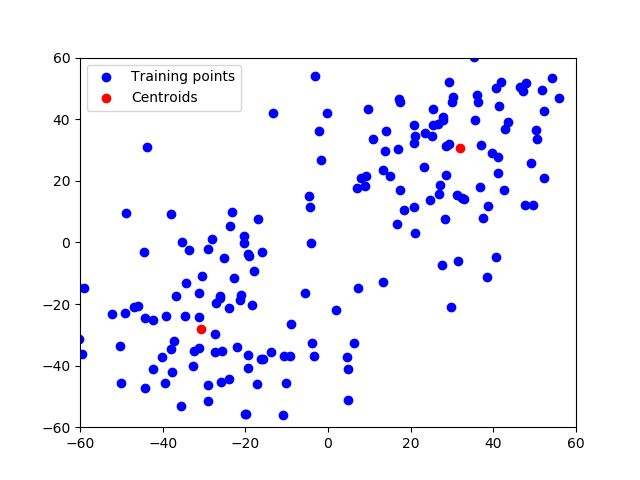
\includegraphics[scale=0.7]{../Immagini/train1.png}
  \caption{Dati generati alla prima generazione del modello}
  \label{fig:train1}
\end{figure}
\begin{figure}[!htb]
  \centering
  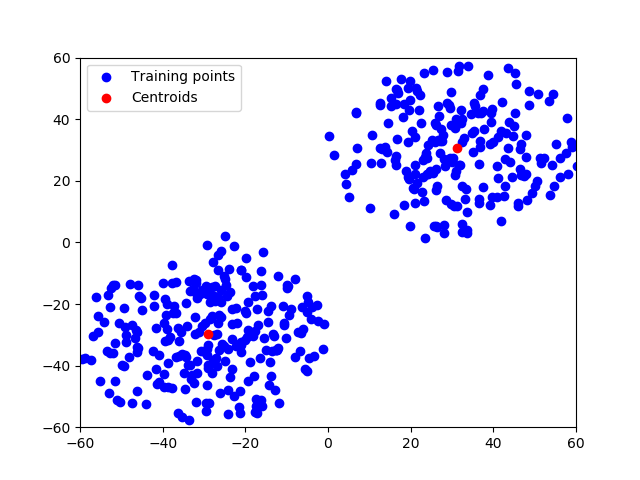
\includegraphics[scale=0.7]{../Immagini/train5.png}
  \caption{Dati generati alla quinta generazione del modello}
  \label{fig:train5}
\end{figure}
\begin{figure}[!htb]
  \centering
  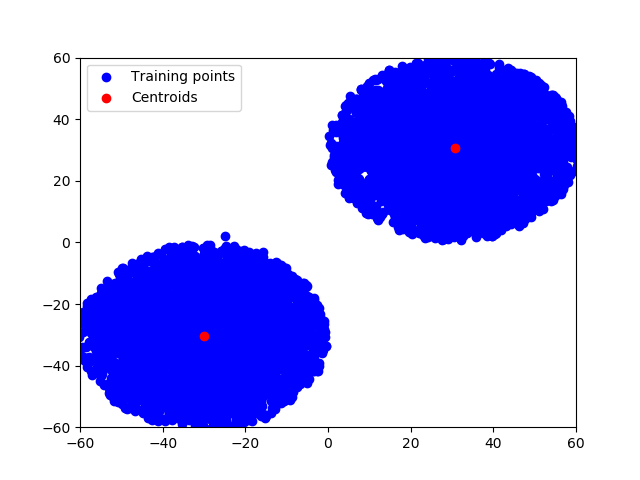
\includegraphics[scale=0.7]{../Immagini/train11.png}
  \caption{Dati generati all'undicesima - e ultima - generazione del modello}
  \label{fig:train11}
\end{figure}
\newpage
\subsection{Unione dei modelli}
Per quanto riguarda l'unione dei modelli il nostro algoritmo si è comportato in accordo alle  figure \ref{fig:merge1},\ref{fig:merge5},\ref{fig:merge11}:
\begin{figure}[!htb]
  \centering
  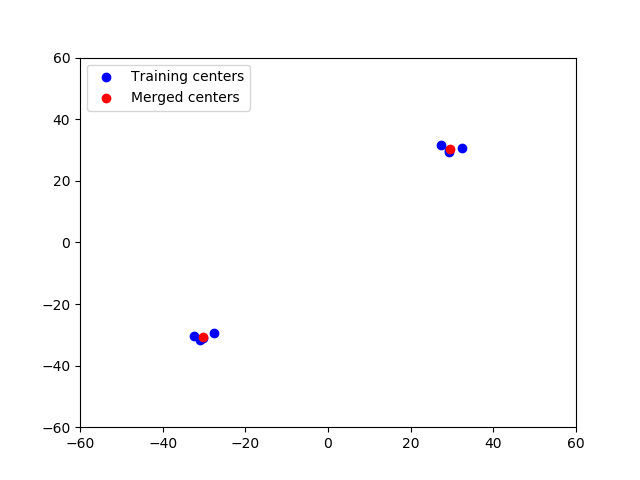
\includegraphics[scale=0.6]{../Immagini/merge1.png}
  \caption{Modelli uniti in seguito alla prima generazione}
  \label{fig:merge1}
\end{figure}
\begin{figure}[!htb]
  \centering
  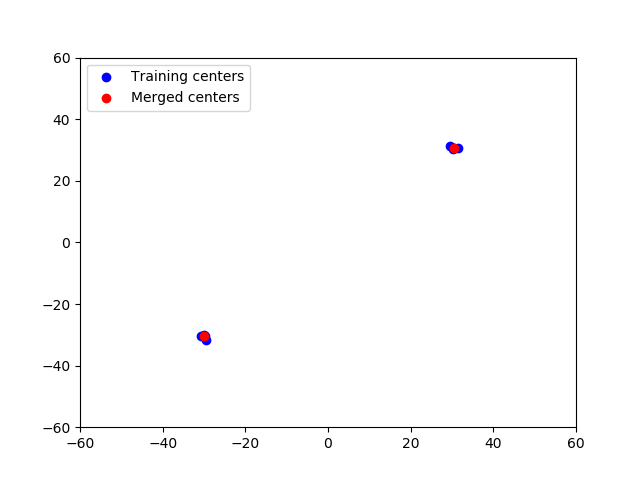
\includegraphics[scale=0.6]{../Immagini/merge5.png}
  \caption{Modelli uniti in seguito alla quinta generazione}
  \label{fig:merge5}
\end{figure}
\begin{figure}[!htb]
  \centering
  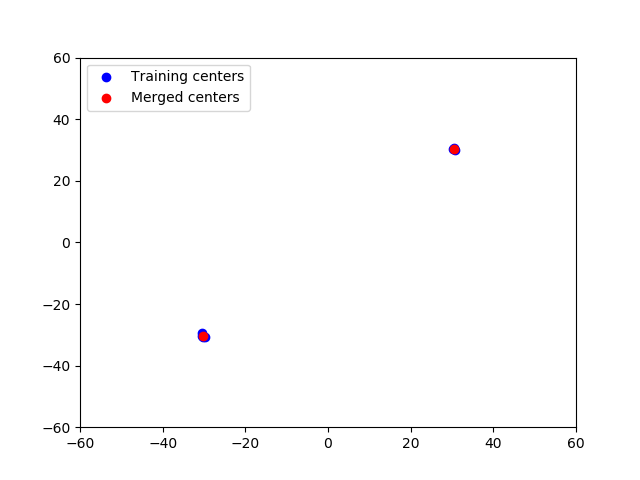
\includegraphics[scale=0.6]{../Immagini/merge11.png}
  \caption{Modelli uniti in seguito alla nona - e ultima - generazione}
  \label{fig:merge11}
\end{figure}


Come si può notare dalle immagini all'aumentare del numero di iterazioni i centri tendono a convergere verso un unico punto, portando quindi ad un modello comune considerabile preciso - in quanto calcolato singolarmente - per tutti i nodi.
\newpage
\subsection{Aggiornamento dei modelli}
Per quanto riguarda l'unione dei modelli il nostro algoritmo si è comportato in accordo alle  figure \ref{fig:update1},\ref{fig:update5},\ref{fig:update9}:
\begin{figure}[!htb]
  \centering
  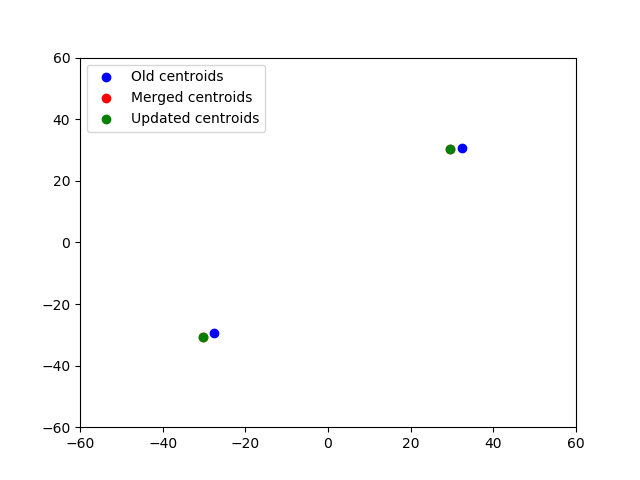
\includegraphics[scale=0.7]{../Immagini/update1.png}
  \caption{Modelli uniti in seguito alla prima generazione}
  \label{fig:update1}
\end{figure}
\begin{figure}[!htb]
  \centering
  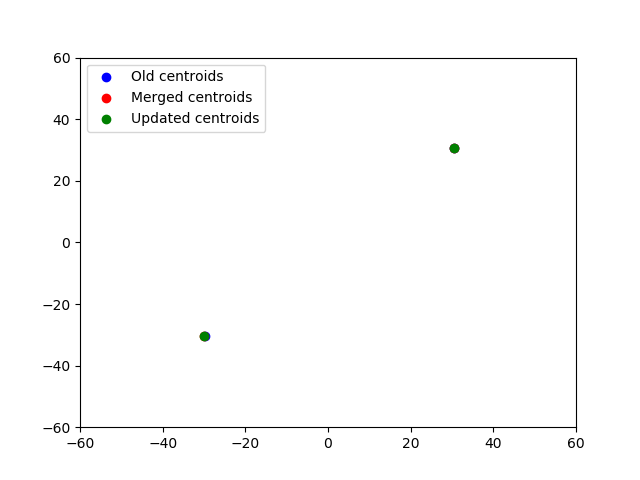
\includegraphics[scale=0.7]{../Immagini/update5.png}
  \caption{Modelli uniti in seguito alla quinta generazione}
  \label{fig:update5}
\end{figure}
\begin{figure}[!htb]
  \centering
  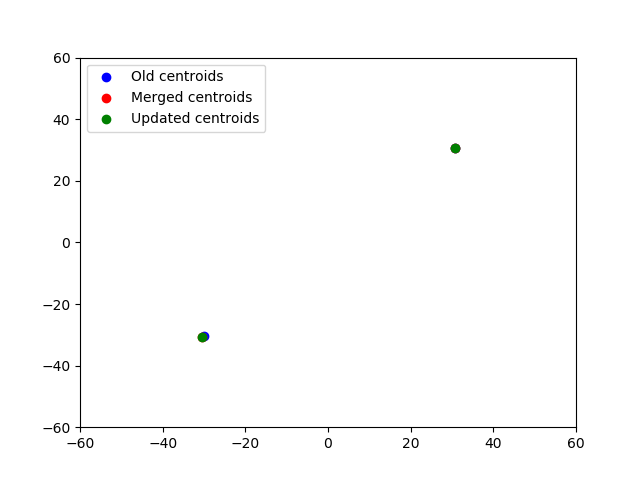
\includegraphics[scale=0.7]{../Immagini/update9.png}
  \caption{Modelli uniti in seguito alla nona - e ultima - generazione}
  \label{fig:update9}
\end{figure}
\newpage
Come si può notare invece da queste figure i punti del modello generati dal nodo erano sempre molto vicini ai punti del modello unificato, ed infatti i punti aggiornati - quelli in verde - si sovrapponevano sempre ai punti del modello unificato - in rosso -.
Si può notare inoltre che lo stesso risultato presentato nell'unione dei modelli si ottiene anche qui, ovvero che i centri del modello generato dal nodo all'aumentare delle iterazioni convergono verso i centri del modello unificato.
